\documentclass[1p]{elsarticle_modified}
%\bibliographystyle{elsarticle-num}

%\usepackage[colorlinks]{hyperref}
%\usepackage{abbrmath_seonhwa} %\Abb, \Ascr, \Acal ,\Abf, \Afrak
\usepackage{amsfonts}
\usepackage{amssymb}
\usepackage{amsmath}
\usepackage{amsthm}
\usepackage{scalefnt}
\usepackage{amsbsy}
\usepackage{kotex}
\usepackage{caption}
\usepackage{subfig}
\usepackage{color}
\usepackage{graphicx}
\usepackage{xcolor} %% white, black, red, green, blue, cyan, magenta, yellow
\usepackage{float}
\usepackage{setspace}
\usepackage{hyperref}

\usepackage{tikz}
\usetikzlibrary{arrows}

\usepackage{multirow}
\usepackage{array} % fixed length table
\usepackage{hhline}

%%%%%%%%%%%%%%%%%%%%%
\makeatletter
\renewcommand*\env@matrix[1][\arraystretch]{%
	\edef\arraystretch{#1}%
	\hskip -\arraycolsep
	\let\@ifnextchar\new@ifnextchar
	\array{*\c@MaxMatrixCols c}}
\makeatother %https://tex.stackexchange.com/questions/14071/how-can-i-increase-the-line-spacing-in-a-matrix
%%%%%%%%%%%%%%%

\usepackage[normalem]{ulem}

\newcommand{\msout}[1]{\ifmmode\text{\sout{\ensuremath{#1}}}\else\sout{#1}\fi}
%SOURCE: \msout is \stkout macro in https://tex.stackexchange.com/questions/20609/strikeout-in-math-mode

\newcommand{\cancel}[1]{
	\ifmmode
	{\color{red}\msout{#1}}
	\else
	{\color{red}\sout{#1}}
	\fi
}

\newcommand{\add}[1]{
	{\color{blue}\uwave{#1}}
}

\newcommand{\replace}[2]{
	\ifmmode
	{\color{red}\msout{#1}}{\color{blue}\uwave{#2}}
	\else
	{\color{red}\sout{#1}}{\color{blue}\uwave{#2}}
	\fi
}

\newcommand{\Sol}{\mathcal{S}} %segment
\newcommand{\D}{D} %diagram
\newcommand{\A}{\mathcal{A}} %arc


%%%%%%%%%%%%%%%%%%%%%%%%%%%%%5 test

\def\sl{\operatorname{\textup{SL}}(2,\Cbb)}
\def\psl{\operatorname{\textup{PSL}}(2,\Cbb)}
\def\quan{\mkern 1mu \triangleright \mkern 1mu}

\theoremstyle{definition}
\newtheorem{thm}{Theorem}[section]
\newtheorem{prop}[thm]{Proposition}
\newtheorem{lem}[thm]{Lemma}
\newtheorem{ques}[thm]{Question}
\newtheorem{cor}[thm]{Corollary}
\newtheorem{defn}[thm]{Definition}
\newtheorem{exam}[thm]{Example}
\newtheorem{rmk}[thm]{Remark}
\newtheorem{alg}[thm]{Algorithm}

\newcommand{\I}{\sqrt{-1}}
\begin{document}

%\begin{frontmatter}
%
%\title{Boundary parabolic representations of knots up to 8 crossings}
%
%%% Group authors per affiliation:
%\author{Yunhi Cho} 
%\address{Department of Mathematics, University of Seoul, Seoul, Korea}
%\ead{yhcho@uos.ac.kr}
%
%
%\author{Seonhwa Kim} %\fnref{s_kim}}
%\address{Center for Geometry and Physics, Institute for Basic Science, Pohang, 37673, Korea}
%\ead{ryeona17@ibs.re.kr}
%
%\author{Hyuk Kim}
%\address{Department of Mathematical Sciences, Seoul National University, Seoul 08826, Korea}
%\ead{hyukkim@snu.ac.kr}
%
%\author{Seokbeom Yoon}
%\address{Department of Mathematical Sciences, Seoul National University, Seoul, 08826,  Korea}
%\ead{sbyoon15@snu.ac.kr}
%
%\begin{abstract}
%We find all boundary parabolic representation of knots up to 8 crossings.
%
%\end{abstract}
%\begin{keyword}
%    \MSC[2010] 57M25 
%\end{keyword}
%
%\end{frontmatter}

%\linenumbers
%\tableofcontents
%
\newcommand\colored[1]{\textcolor{white}{\rule[-0.35ex]{0.8em}{1.4ex}}\kern-0.8em\color{red} #1}%
%\newcommand\colored[1]{\textcolor{white}{ #1}\kern-2.17ex	\textcolor{white}{ #1}\kern-1.81ex	\textcolor{white}{ #1}\kern-2.15ex\color{red}#1	}

{\Large $\underline{12a_{0168}~(K12a_{0168})}$}

\setlength{\tabcolsep}{10pt}
\renewcommand{\arraystretch}{1.6}
\vspace{1cm}\begin{tabular}{m{100pt}>{\centering\arraybackslash}m{274pt}}
\multirow{5}{120pt}{
	\centering
	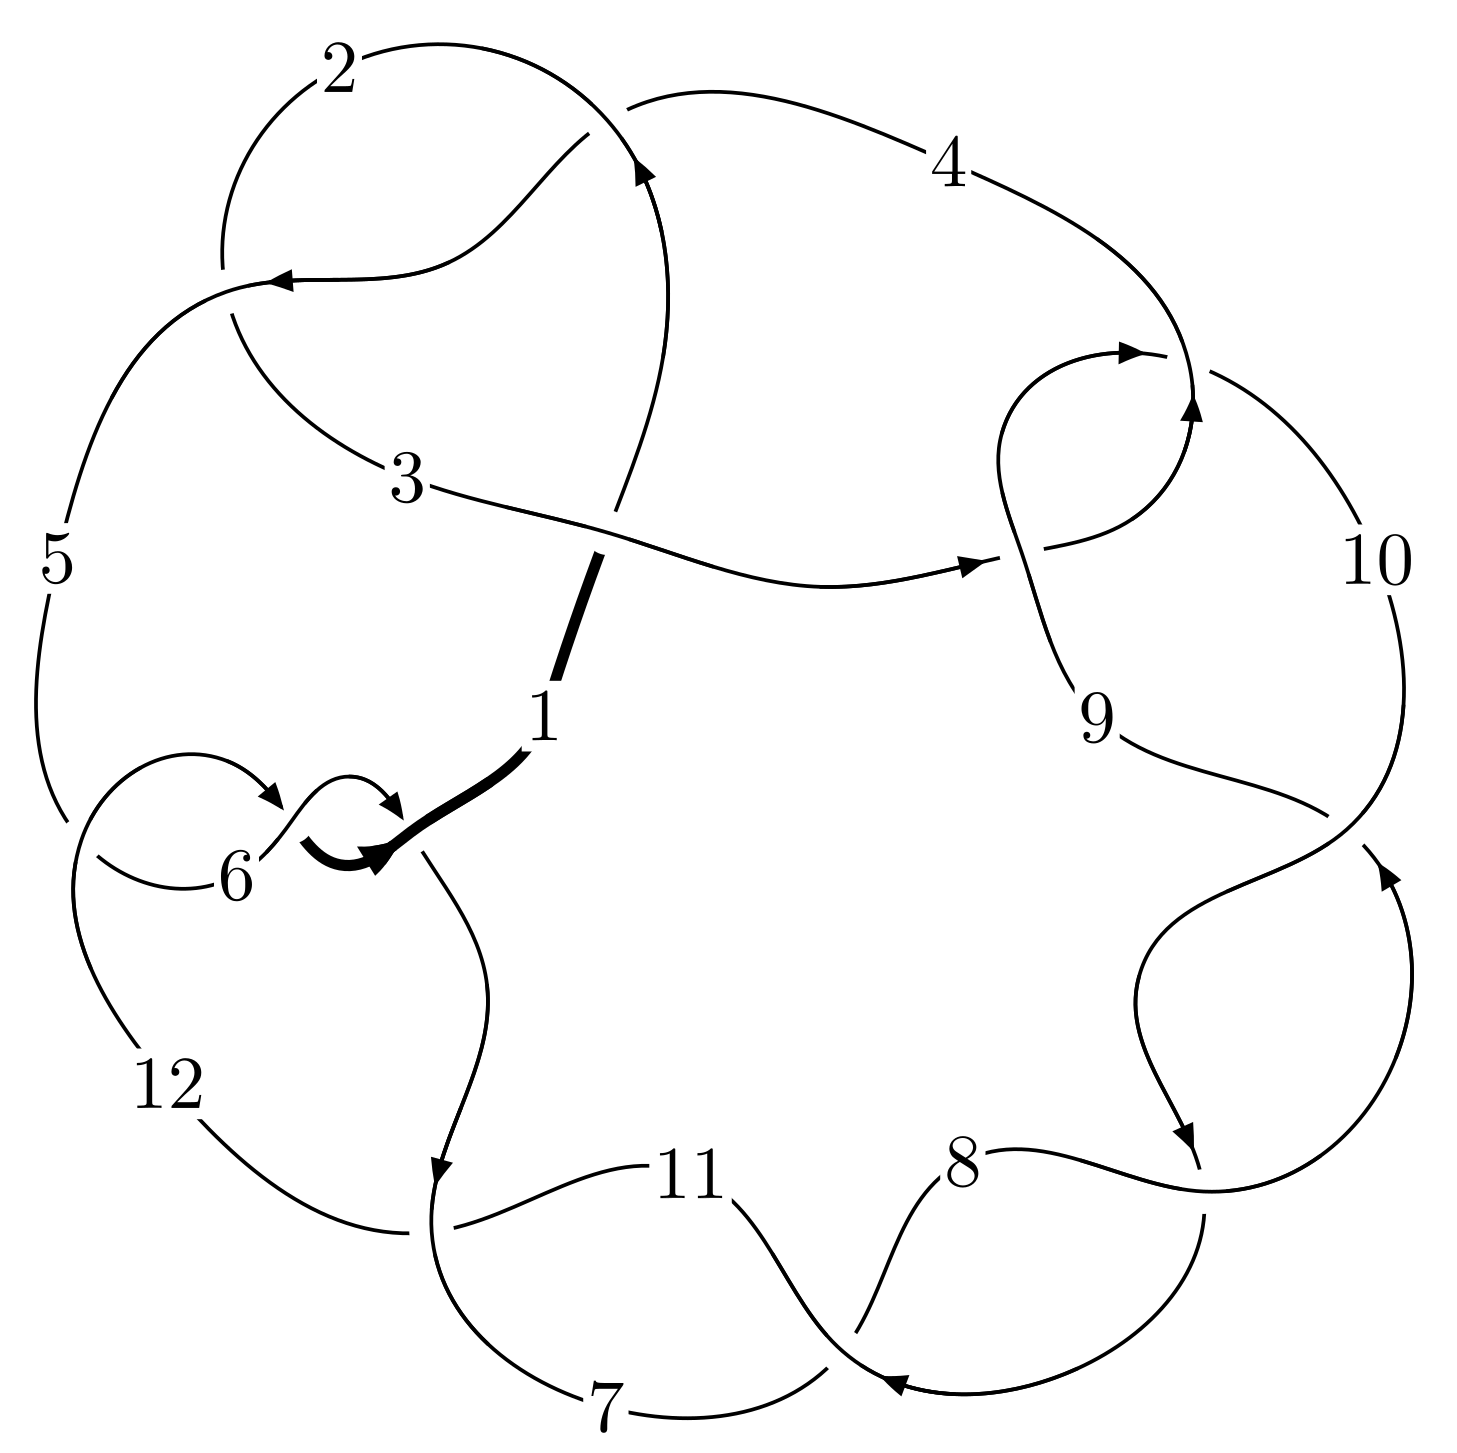
\includegraphics[width=112pt]{../../../GIT/diagram.site/Diagrams/png/969_12a_0168.png}\\
\ \ \ A knot diagram\footnotemark}&
\allowdisplaybreaks
\textbf{Linearized knot diagam} \\
\cline{2-2}
 &
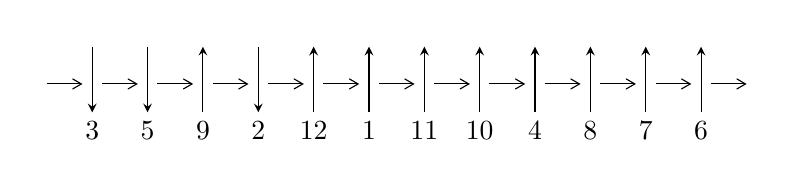
\begin{tikzpicture}[x=20pt, y=17pt]
	% nodes
	\node (C0) at (0, 0) {};
	\node (C1) at (1, 0) {};
	\node (C1U) at (1, +1) {};
	\node (C1D) at (1, -1) {3};

	\node (C2) at (2, 0) {};
	\node (C2U) at (2, +1) {};
	\node (C2D) at (2, -1) {5};

	\node (C3) at (3, 0) {};
	\node (C3U) at (3, +1) {};
	\node (C3D) at (3, -1) {9};

	\node (C4) at (4, 0) {};
	\node (C4U) at (4, +1) {};
	\node (C4D) at (4, -1) {2};

	\node (C5) at (5, 0) {};
	\node (C5U) at (5, +1) {};
	\node (C5D) at (5, -1) {12};

	\node (C6) at (6, 0) {};
	\node (C6U) at (6, +1) {};
	\node (C6D) at (6, -1) {1};

	\node (C7) at (7, 0) {};
	\node (C7U) at (7, +1) {};
	\node (C7D) at (7, -1) {11};

	\node (C8) at (8, 0) {};
	\node (C8U) at (8, +1) {};
	\node (C8D) at (8, -1) {10};

	\node (C9) at (9, 0) {};
	\node (C9U) at (9, +1) {};
	\node (C9D) at (9, -1) {4};

	\node (C10) at (10, 0) {};
	\node (C10U) at (10, +1) {};
	\node (C10D) at (10, -1) {8};

	\node (C11) at (11, 0) {};
	\node (C11U) at (11, +1) {};
	\node (C11D) at (11, -1) {7};

	\node (C12) at (12, 0) {};
	\node (C12U) at (12, +1) {};
	\node (C12D) at (12, -1) {6};
	\node (C13) at (13, 0) {};

	% arrows
	\draw[->,>={angle 60}]
	(C0) edge (C1) (C1) edge (C2) (C2) edge (C3) (C3) edge (C4) (C4) edge (C5) (C5) edge (C6) (C6) edge (C7) (C7) edge (C8) (C8) edge (C9) (C9) edge (C10) (C10) edge (C11) (C11) edge (C12) (C12) edge (C13) ;	\draw[->,>=stealth]
	(C1U) edge (C1D) (C2U) edge (C2D) (C3D) edge (C3U) (C4U) edge (C4D) (C5D) edge (C5U) (C6D) edge (C6U) (C7D) edge (C7U) (C8D) edge (C8U) (C9D) edge (C9U) (C10D) edge (C10U) (C11D) edge (C11U) (C12D) edge (C12U) ;
	\end{tikzpicture} \\
\hhline{~~} \\& 
\textbf{Solving Sequence} \\ \cline{2-2} 
 &
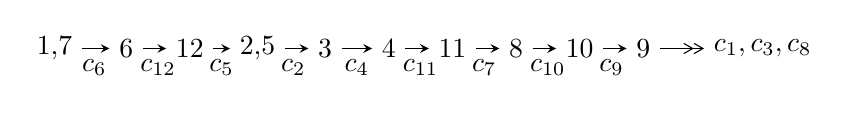
\begin{tikzpicture}[x=23pt, y=7pt]
	% node
	\node (A0) at (-1/8, 0) {1,7};
	\node (A1) at (1, 0) {6};
	\node (A2) at (2, 0) {12};
	\node (A3) at (49/16, 0) {2,5};
	\node (A4) at (33/8, 0) {3};
	\node (A5) at (41/8, 0) {4};
	\node (A6) at (49/8, 0) {11};
	\node (A7) at (57/8, 0) {8};
	\node (A8) at (65/8, 0) {10};
	\node (A9) at (73/8, 0) {9};
	\node (C1) at (1/2, -1) {$c_{6}$};
	\node (C2) at (3/2, -1) {$c_{12}$};
	\node (C3) at (5/2, -1) {$c_{5}$};
	\node (C4) at (29/8, -1) {$c_{2}$};
	\node (C5) at (37/8, -1) {$c_{4}$};
	\node (C6) at (45/8, -1) {$c_{11}$};
	\node (C7) at (53/8, -1) {$c_{7}$};
	\node (C8) at (61/8, -1) {$c_{10}$};
	\node (C9) at (69/8, -1) {$c_{9}$};
	\node (A10) at (11, 0) {$c_{1},c_{3},c_{8}$};

	% edge
	\draw[->,>=stealth]	
	(A0) edge (A1) (A1) edge (A2) (A2) edge (A3) (A3) edge (A4) (A4) edge (A5) (A5) edge (A6) (A6) edge (A7) (A7) edge (A8) (A8) edge (A9) ;
	\draw[->>,>={angle 60}]	
	(A9) edge (A10);
\end{tikzpicture} \\ 

\end{tabular} \\

\footnotetext{
The image of knot diagram is generated by the software ``\textbf{Draw programme}" developed by Andrew Bartholomew(\url{http://www.layer8.co.uk/maths/draw/index.htm\#Running-draw}), where we modified some parts for our purpose(\url{https://github.com/CATsTAILs/LinksPainter}).
}\phantom \\ \newline 
\centering \textbf{Ideals for irreducible components\footnotemark of $X_{\text{par}}$} 
 
\begin{align*}
I^u_{1}&=\langle 
- u^{28}+10 u^{26}+\cdots+6 u^2+b,\;- u^{34}+u^{33}+\cdots+a-8 u,\;u^{35}-2 u^{34}+\cdots- u+1\rangle \\
I^u_{2}&=\langle 
u^5- u^3+b- u,\;u^3+a,\\
\phantom{I^u_{2}}&\phantom{= \langle  }u^{15}-5 u^{13}- u^{12}+10 u^{11}+4 u^{10}-6 u^9-6 u^8-7 u^7+u^6+11 u^5+5 u^4- u^3-3 u^2-3 u-1\rangle \\
I^u_{3}&=\langle 
b+1,\;a-1,\;u+1\rangle \\
\\
\end{align*}
\raggedright * 3 irreducible components of $\dim_{\mathbb{C}}=0$, with total 51 representations.\\
\footnotetext{All coefficients of polynomials are rational numbers. But the coefficients are sometimes approximated in decimal forms when there is not enough margin.}
\newpage
\renewcommand{\arraystretch}{1}
\centering \section*{I. $I^u_{1}= \langle - u^{28}+10 u^{26}+\cdots+6 u^2+b,\;- u^{34}+u^{33}+\cdots+a-8 u,\;u^{35}-2 u^{34}+\cdots- u+1 \rangle$}
\flushleft \textbf{(i) Arc colorings}\\
\begin{tabular}{m{7pt} m{180pt} m{7pt} m{180pt} }
\flushright $a_{1}=$&$\begin{pmatrix}0\\u\end{pmatrix}$ \\
\flushright $a_{7}=$&$\begin{pmatrix}1\\0\end{pmatrix}$ \\
\flushright $a_{6}=$&$\begin{pmatrix}1\\u^2\end{pmatrix}$ \\
\flushright $a_{12}=$&$\begin{pmatrix}- u\\- u^3+u\end{pmatrix}$ \\
\flushright $a_{2}=$&$\begin{pmatrix}u^{34}- u^{33}+\cdots+20 u^2+8 u\\u^{28}-10 u^{26}+\cdots-16 u^3-6 u^2\end{pmatrix}$ \\
\flushright $a_{5}=$&$\begin{pmatrix}- u^2+1\\- u^4+2 u^2\end{pmatrix}$ \\
\flushright $a_{3}=$&$\begin{pmatrix}- u^{33}+13 u^{31}+\cdots+28 u^2+8 u\\- u^{34}+u^{33}+\cdots- u+1\end{pmatrix}$ \\
\flushright $a_{4}=$&$\begin{pmatrix}u^{34}-13 u^{32}+\cdots-7 u-1\\u^{34}- u^{33}+\cdots+u-1\end{pmatrix}$ \\
\flushright $a_{11}=$&$\begin{pmatrix}u^3-2 u\\- u^3+u\end{pmatrix}$ \\
\flushright $a_{8}=$&$\begin{pmatrix}u^6-3 u^4+2 u^2+1\\- u^6+2 u^4- u^2\end{pmatrix}$ \\
\flushright $a_{10}=$&$\begin{pmatrix}u^9-4 u^7+5 u^5-3 u\\- u^9+3 u^7-3 u^5+u\end{pmatrix}$ \\
\flushright $a_{9}=$&$\begin{pmatrix}u^{12}-5 u^{10}+9 u^8-4 u^6-6 u^4+5 u^2+1\\- u^{12}+4 u^{10}-6 u^8+2 u^6+3 u^4-2 u^2\end{pmatrix}$\\&\end{tabular}
\flushleft \textbf{(ii) Obstruction class $= -1$}\\~\\
\flushleft \textbf{(iii) Cusp Shapes $= -2 u^{33}+4 u^{32}+26 u^{31}-48 u^{30}-154 u^{29}+252 u^{28}+536 u^{27}-724 u^{26}-1162 u^{25}+1096 u^{24}+1448 u^{23}-336 u^{22}-448 u^{21}-1792 u^{20}-1708 u^{19}+2984 u^{18}+2926 u^{17}-836 u^{16}-1400 u^{15}-2388 u^{14}-1280 u^{13}+2228 u^{12}+1868 u^{11}+404 u^{10}-328 u^9-1140 u^8-596 u^7+60 u^6+196 u^5+236 u^4+100 u^3+28 u^2-6 u$}\\~\\
\newpage\renewcommand{\arraystretch}{1}
\flushleft \textbf{(iv) u-Polynomials at the component}\newline \\
\begin{tabular}{m{50pt}|m{274pt}}
Crossings & \hspace{64pt}u-Polynomials at each crossing \\
\hline $$\begin{aligned}c_{1}\end{aligned}$$&$\begin{aligned}
&u^{35}+20 u^{34}+\cdots+3 u+1
\end{aligned}$\\
\hline $$\begin{aligned}c_{2},c_{4}\end{aligned}$$&$\begin{aligned}
&u^{35}-2 u^{34}+\cdots+3 u-1
\end{aligned}$\\
\hline $$\begin{aligned}c_{3},c_{9}\end{aligned}$$&$\begin{aligned}
&u^{35}+2 u^{34}+\cdots-2 u-2
\end{aligned}$\\
\hline $$\begin{aligned}c_{5},c_{6},c_{12}\end{aligned}$$&$\begin{aligned}
&u^{35}+2 u^{34}+\cdots- u-1
\end{aligned}$\\
\hline $$\begin{aligned}c_{7},c_{8},c_{10}\\c_{11}\end{aligned}$$&$\begin{aligned}
&u^{35}-6 u^{34}+\cdots+8 u-4
\end{aligned}$\\
\hline
\end{tabular}\\~\\
\newpage\renewcommand{\arraystretch}{1}
\flushleft \textbf{(v) Riley Polynomials at the component}\newline \\
\begin{tabular}{m{50pt}|m{274pt}}
Crossings & \hspace{64pt}Riley Polynomials at each crossing \\
\hline $$\begin{aligned}c_{1}\end{aligned}$$&$\begin{aligned}
&y^{35}-8 y^{34}+\cdots+35 y-1
\end{aligned}$\\
\hline $$\begin{aligned}c_{2},c_{4}\end{aligned}$$&$\begin{aligned}
&y^{35}-20 y^{34}+\cdots+3 y-1
\end{aligned}$\\
\hline $$\begin{aligned}c_{3},c_{9}\end{aligned}$$&$\begin{aligned}
&y^{35}-6 y^{34}+\cdots+8 y-4
\end{aligned}$\\
\hline $$\begin{aligned}c_{5},c_{6},c_{12}\end{aligned}$$&$\begin{aligned}
&y^{35}-28 y^{34}+\cdots-13 y-1
\end{aligned}$\\
\hline $$\begin{aligned}c_{7},c_{8},c_{10}\\c_{11}\end{aligned}$$&$\begin{aligned}
&y^{35}+42 y^{34}+\cdots-136 y-16
\end{aligned}$\\
\hline
\end{tabular}\\~\\
\newpage\flushleft \textbf{(vi) Complex Volumes and Cusp Shapes}
$$\begin{array}{c|c|c}  
\text{Solutions to }I^u_{1}& \I (\text{vol} + \sqrt{-1}CS) & \text{Cusp shape}\\
 \hline 
\begin{aligned}
u &= -0.029628 + 0.934102 I \\
a &= -3.61963 + 0.54565 I \\
b &= \phantom{-}4.19510 - 0.71037 I\end{aligned}
 & -14.7947 - 8.3253 I & -0.91975 + 5.31258 I \\ \hline\begin{aligned}
u &= -0.029628 - 0.934102 I \\
a &= -3.61963 - 0.54565 I \\
b &= \phantom{-}4.19510 + 0.71037 I\end{aligned}
 & -14.7947 + 8.3253 I & -0.91975 - 5.31258 I \\ \hline\begin{aligned}
u &= \phantom{-}0.004692 + 0.923942 I \\
a &= \phantom{-}3.64319 + 0.66960 I \\
b &= -4.10450 - 1.08656 I\end{aligned}
 & -14.9356 + 1.5707 I & -1.236325 - 0.670783 I \\ \hline\begin{aligned}
u &= \phantom{-}0.004692 - 0.923942 I \\
a &= \phantom{-}3.64319 - 0.66960 I \\
b &= -4.10450 + 1.08656 I\end{aligned}
 & -14.9356 - 1.5707 I & -1.236325 + 0.670783 I \\ \hline\begin{aligned}
u &= -1.140910 + 0.226464 I \\
a &= \phantom{-}0.0410600 + 0.0527107 I \\
b &= -0.796518 + 0.135470 I\end{aligned}
 & \phantom{-}1.16280 - 0.99874 I & \phantom{-}6.67808 + 0.23087 I \\ \hline\begin{aligned}
u &= -1.140910 - 0.226464 I \\
a &= \phantom{-}0.0410600 - 0.0527107 I \\
b &= -0.796518 - 0.135470 I\end{aligned}
 & \phantom{-}1.16280 + 0.99874 I & \phantom{-}6.67808 - 0.23087 I \\ \hline\begin{aligned}
u &= -1.211370 + 0.063006 I \\
a &= -0.024848 + 0.395141 I \\
b &= -0.93931 - 1.68300 I\end{aligned}
 & \phantom{-}2.16189 - 1.54722 I & \phantom{-}7.54202 + 4.01814 I \\ \hline\begin{aligned}
u &= -1.211370 - 0.063006 I \\
a &= -0.024848 - 0.395141 I \\
b &= -0.93931 + 1.68300 I\end{aligned}
 & \phantom{-}2.16189 + 1.54722 I & \phantom{-}7.54202 - 4.01814 I \\ \hline\begin{aligned}
u &= -0.139390 + 0.744521 I \\
a &= -2.63405 + 0.70052 I \\
b &= \phantom{-}1.81184 - 0.03604 I\end{aligned}
 & -4.64613 - 6.27110 I & \phantom{-}0.28899 + 7.66392 I \\ \hline\begin{aligned}
u &= -0.139390 - 0.744521 I \\
a &= -2.63405 - 0.70052 I \\
b &= \phantom{-}1.81184 + 0.03604 I\end{aligned}
 & -4.64613 + 6.27110 I & \phantom{-}0.28899 - 7.66392 I\\
 \hline 
 \end{array}$$\newpage$$\begin{array}{c|c|c}  
\text{Solutions to }I^u_{1}& \I (\text{vol} + \sqrt{-1}CS) & \text{Cusp shape}\\
 \hline 
\begin{aligned}
u &= -1.233890 + 0.279365 I \\
a &= -0.14304 + 1.43122 I \\
b &= \phantom{-}2.18803 - 1.44880 I\end{aligned}
 & -1.47413 - 4.67753 I & \phantom{-}3.26707 + 4.95430 I \\ \hline\begin{aligned}
u &= -1.233890 - 0.279365 I \\
a &= -0.14304 - 1.43122 I \\
b &= \phantom{-}2.18803 + 1.44880 I\end{aligned}
 & -1.47413 + 4.67753 I & \phantom{-}3.26707 - 4.95430 I \\ \hline\begin{aligned}
u &= \phantom{-}1.276390 + 0.259219 I \\
a &= -0.047693 + 0.240818 I \\
b &= \phantom{-}0.432237 + 0.227863 I\end{aligned}
 & \phantom{-}2.43611 + 5.45580 I & \phantom{-}9.29163 - 6.05568 I \\ \hline\begin{aligned}
u &= \phantom{-}1.276390 - 0.259219 I \\
a &= -0.047693 - 0.240818 I \\
b &= \phantom{-}0.432237 - 0.227863 I\end{aligned}
 & \phantom{-}2.43611 - 5.45580 I & \phantom{-}9.29163 + 6.05568 I \\ \hline\begin{aligned}
u &= \phantom{-}1.302250 + 0.054350 I \\
a &= \phantom{-}0.287821 - 0.006470 I \\
b &= \phantom{-}0.723841 + 0.741201 I\end{aligned}
 & \phantom{-}6.06693 + 0.68963 I & \phantom{-}14.6543 - 0.4108 I \\ \hline\begin{aligned}
u &= \phantom{-}1.302250 - 0.054350 I \\
a &= \phantom{-}0.287821 + 0.006470 I \\
b &= \phantom{-}0.723841 - 0.741201 I\end{aligned}
 & \phantom{-}6.06693 - 0.68963 I & \phantom{-}14.6543 + 0.4108 I \\ \hline\begin{aligned}
u &= \phantom{-}1.314130 + 0.126505 I \\
a &= \phantom{-}0.477565 + 0.637528 I \\
b &= -0.035059 - 0.928052 I\end{aligned}
 & \phantom{-}5.18133 + 4.97391 I & \phantom{-}11.84206 - 7.53779 I \\ \hline\begin{aligned}
u &= \phantom{-}1.314130 - 0.126505 I \\
a &= \phantom{-}0.477565 - 0.637528 I \\
b &= -0.035059 + 0.928052 I\end{aligned}
 & \phantom{-}5.18133 - 4.97391 I & \phantom{-}11.84206 + 7.53779 I \\ \hline\begin{aligned}
u &= \phantom{-}0.028586 + 0.673943 I \\
a &= \phantom{-}2.75743 + 1.25369 I \\
b &= -1.39032 - 1.02302 I\end{aligned}
 & -5.31953 + 1.23761 I & -2.13192 - 0.75441 I \\ \hline\begin{aligned}
u &= \phantom{-}0.028586 - 0.673943 I \\
a &= \phantom{-}2.75743 - 1.25369 I \\
b &= -1.39032 + 1.02302 I\end{aligned}
 & -5.31953 - 1.23761 I & -2.13192 + 0.75441 I\\
 \hline 
 \end{array}$$\newpage$$\begin{array}{c|c|c}  
\text{Solutions to }I^u_{1}& \I (\text{vol} + \sqrt{-1}CS) & \text{Cusp shape}\\
 \hline 
\begin{aligned}
u &= \phantom{-}1.306990 + 0.302770 I \\
a &= \phantom{-}0.54892 + 1.54089 I \\
b &= -2.14001 - 0.30607 I\end{aligned}
 & -0.13672 + 10.00530 I & \phantom{-}5.74688 - 9.45823 I \\ \hline\begin{aligned}
u &= \phantom{-}1.306990 - 0.302770 I \\
a &= \phantom{-}0.54892 - 1.54089 I \\
b &= -2.14001 + 0.30607 I\end{aligned}
 & -0.13672 - 10.00530 I & \phantom{-}5.74688 + 9.45823 I \\ \hline\begin{aligned}
u &= -1.274370 + 0.449256 I \\
a &= \phantom{-}0.464706 + 0.179729 I \\
b &= -0.289894 - 0.612925 I\end{aligned}
 & -7.05845 - 1.54689 I & \phantom{-}5.29634 + 0.63495 I \\ \hline\begin{aligned}
u &= -1.274370 - 0.449256 I \\
a &= \phantom{-}0.464706 - 0.179729 I \\
b &= -0.289894 + 0.612925 I\end{aligned}
 & -7.05845 + 1.54689 I & \phantom{-}5.29634 - 0.63495 I \\ \hline\begin{aligned}
u &= -1.292980 + 0.447168 I \\
a &= -0.48290 + 2.40208 I \\
b &= \phantom{-}4.44596 + 0.24017 I\end{aligned}
 & -10.90240 - 6.46399 I & \phantom{-}2.13256 + 3.64968 I \\ \hline\begin{aligned}
u &= -1.292980 - 0.447168 I \\
a &= -0.48290 - 2.40208 I \\
b &= \phantom{-}4.44596 - 0.24017 I\end{aligned}
 & -10.90240 + 6.46399 I & \phantom{-}2.13256 - 3.64968 I \\ \hline\begin{aligned}
u &= \phantom{-}1.300000 + 0.439361 I \\
a &= -0.464718 + 0.254925 I \\
b &= \phantom{-}0.131131 - 0.562319 I\end{aligned}
 & -6.86104 + 8.18007 I & \phantom{-}5.63732 - 5.18856 I \\ \hline\begin{aligned}
u &= \phantom{-}1.300000 - 0.439361 I \\
a &= -0.464718 - 0.254925 I \\
b &= \phantom{-}0.131131 + 0.562319 I\end{aligned}
 & -6.86104 - 8.18007 I & \phantom{-}5.63732 + 5.18856 I \\ \hline\begin{aligned}
u &= \phantom{-}1.313670 + 0.446415 I \\
a &= \phantom{-}0.61332 + 2.40054 I \\
b &= -4.34015 + 0.59580 I\end{aligned}
 & -10.6081 + 13.2523 I & \phantom{-}2.64420 - 8.00654 I \\ \hline\begin{aligned}
u &= \phantom{-}1.313670 - 0.446415 I \\
a &= \phantom{-}0.61332 - 2.40054 I \\
b &= -4.34015 - 0.59580 I\end{aligned}
 & -10.6081 - 13.2523 I & \phantom{-}2.64420 + 8.00654 I\\
 \hline 
 \end{array}$$\newpage$$\begin{array}{c|c|c}  
\text{Solutions to }I^u_{1}& \I (\text{vol} + \sqrt{-1}CS) & \text{Cusp shape}\\
 \hline 
\begin{aligned}
u &= -0.605125\phantom{ +0.000000I} \\
a &= \phantom{-}0.150256\phantom{ +0.000000I} \\
b &= -0.724538\phantom{ +0.000000I}\end{aligned}
 & \phantom{-}0.878305\phantom{ +0.000000I} & \phantom{-}11.8450\phantom{ +0.000000I} \\ \hline\begin{aligned}
u &= -0.357155 + 0.473523 I \\
a &= -1.032500 + 0.775837 I \\
b &= -0.077318 + 0.333065 I\end{aligned}
 & \phantom{-}0.06389 - 3.04882 I & \phantom{-}6.31761 + 9.14792 I \\ \hline\begin{aligned}
u &= -0.357155 - 0.473523 I \\
a &= -1.032500 - 0.775837 I \\
b &= -0.077318 - 0.333065 I\end{aligned}
 & \phantom{-}0.06389 + 3.04882 I & \phantom{-}6.31761 - 9.14792 I \\ \hline\begin{aligned}
u &= \phantom{-}0.135558 + 0.221933 I \\
a &= \phantom{-}0.04024 + 3.17604 I \\
b &= \phantom{-}0.547219 - 0.274542 I\end{aligned}
 & -1.63800 + 0.52732 I & -3.97358 - 0.67184 I \\ \hline\begin{aligned}
u &= \phantom{-}0.135558 - 0.221933 I \\
a &= \phantom{-}0.04024 - 3.17604 I \\
b &= \phantom{-}0.547219 + 0.274542 I\end{aligned}
 & -1.63800 - 0.52732 I & -3.97358 + 0.67184 I\\
 \hline 
 \end{array}$$\newpage\newpage\renewcommand{\arraystretch}{1}
\centering \section*{II. $I^u_{2}= \langle u^5- u^3+b- u,\;u^3+a,\;u^{15}-5 u^{13}+\cdots-3 u-1 \rangle$}
\flushleft \textbf{(i) Arc colorings}\\
\begin{tabular}{m{7pt} m{180pt} m{7pt} m{180pt} }
\flushright $a_{1}=$&$\begin{pmatrix}0\\u\end{pmatrix}$ \\
\flushright $a_{7}=$&$\begin{pmatrix}1\\0\end{pmatrix}$ \\
\flushright $a_{6}=$&$\begin{pmatrix}1\\u^2\end{pmatrix}$ \\
\flushright $a_{12}=$&$\begin{pmatrix}- u\\- u^3+u\end{pmatrix}$ \\
\flushright $a_{2}=$&$\begin{pmatrix}- u^3\\- u^5+u^3+u\end{pmatrix}$ \\
\flushright $a_{5}=$&$\begin{pmatrix}- u^2+1\\- u^4+2 u^2\end{pmatrix}$ \\
\flushright $a_{3}=$&$\begin{pmatrix}- u\\- u^3+u\end{pmatrix}$ \\
\flushright $a_{4}=$&$\begin{pmatrix}u^4- u^2+1\\u^6-2 u^4+u^2\end{pmatrix}$ \\
\flushright $a_{11}=$&$\begin{pmatrix}u^3-2 u\\- u^3+u\end{pmatrix}$ \\
\flushright $a_{8}=$&$\begin{pmatrix}u^6-3 u^4+2 u^2+1\\- u^6+2 u^4- u^2\end{pmatrix}$ \\
\flushright $a_{10}=$&$\begin{pmatrix}u^9-4 u^7+5 u^5-3 u\\- u^9+3 u^7-3 u^5+u\end{pmatrix}$ \\
\flushright $a_{9}=$&$\begin{pmatrix}u^{12}-5 u^{10}+9 u^8-4 u^6-6 u^4+5 u^2+1\\- u^{12}+4 u^{10}-6 u^8+2 u^6+3 u^4-2 u^2\end{pmatrix}$\\&\end{tabular}
\flushleft \textbf{(ii) Obstruction class $= -1$}\\~\\
\flushleft \textbf{(iii) Cusp Shapes $= 4 u^{12}-16 u^{10}-4 u^9+24 u^8+12 u^7-12 u^5-28 u^4-8 u^3+16 u^2+12 u+14$}\\~\\
\newpage\renewcommand{\arraystretch}{1}
\flushleft \textbf{(iv) u-Polynomials at the component}\newline \\
\begin{tabular}{m{50pt}|m{274pt}}
Crossings & \hspace{64pt}u-Polynomials at each crossing \\
\hline $$\begin{aligned}c_{1}\end{aligned}$$&$\begin{aligned}
&u^{15}+10 u^{14}+\cdots+3 u+1
\end{aligned}$\\
\hline $$\begin{aligned}c_{2},c_{4},c_{5}\\c_{6},c_{12}\end{aligned}$$&$\begin{aligned}
&u^{15}-5 u^{13}+\cdots-3 u+1
\end{aligned}$\\
\hline $$\begin{aligned}c_{3},c_{9}\end{aligned}$$&$\begin{aligned}
&(u^5- u^4+u^2+u-1)^3
\end{aligned}$\\
\hline $$\begin{aligned}c_{7},c_{8},c_{10}\\c_{11}\end{aligned}$$&$\begin{aligned}
&(u^5- u^4+4 u^3-3 u^2+3 u-1)^3
\end{aligned}$\\
\hline
\end{tabular}\\~\\
\newpage\renewcommand{\arraystretch}{1}
\flushleft \textbf{(v) Riley Polynomials at the component}\newline \\
\begin{tabular}{m{50pt}|m{274pt}}
Crossings & \hspace{64pt}Riley Polynomials at each crossing \\
\hline $$\begin{aligned}c_{1}\end{aligned}$$&$\begin{aligned}
&y^{15}-10 y^{14}+\cdots+23 y-1
\end{aligned}$\\
\hline $$\begin{aligned}c_{2},c_{4},c_{5}\\c_{6},c_{12}\end{aligned}$$&$\begin{aligned}
&y^{15}-10 y^{14}+\cdots+3 y-1
\end{aligned}$\\
\hline $$\begin{aligned}c_{3},c_{9}\end{aligned}$$&$\begin{aligned}
&(y^5- y^4+4 y^3-3 y^2+3 y-1)^3
\end{aligned}$\\
\hline $$\begin{aligned}c_{7},c_{8},c_{10}\\c_{11}\end{aligned}$$&$\begin{aligned}
&(y^5+7 y^4+16 y^3+13 y^2+3 y-1)^3
\end{aligned}$\\
\hline
\end{tabular}\\~\\
\newpage\flushleft \textbf{(vi) Complex Volumes and Cusp Shapes}
$$\begin{array}{c|c|c}  
\text{Solutions to }I^u_{2}& \I (\text{vol} + \sqrt{-1}CS) & \text{Cusp shape}\\
 \hline 
\begin{aligned}
u &= -0.016489 + 0.918115 I \\
a &= -0.041693 + 0.773164 I \\
b &= \phantom{-}0.083746 - 0.505303 I\end{aligned}
 & -10.95830 - 3.33174 I & \phantom{-}2.08126 + 2.36228 I \\ \hline\begin{aligned}
u &= -0.016489 - 0.918115 I \\
a &= -0.041693 - 0.773164 I \\
b &= \phantom{-}0.083746 + 0.505303 I\end{aligned}
 & -10.95830 + 3.33174 I & \phantom{-}2.08126 - 2.36228 I \\ \hline\begin{aligned}
u &= -1.088950 + 0.365332 I \\
a &= \phantom{-}0.85527 - 1.25089 I \\
b &= -2.03946 - 0.38065 I\end{aligned}
 & -1.81981 + 2.21397 I & \phantom{-}3.11432 - 4.22289 I \\ \hline\begin{aligned}
u &= -1.088950 - 0.365332 I \\
a &= \phantom{-}0.85527 + 1.25089 I \\
b &= -2.03946 + 0.38065 I\end{aligned}
 & -1.81981 - 2.21397 I & \phantom{-}3.11432 + 4.22289 I \\ \hline\begin{aligned}
u &= \phantom{-}1.16504\phantom{ +0.000000I} \\
a &= -1.58132\phantom{ +0.000000I} \\
b &= \phantom{-}0.600011\phantom{ +0.000000I}\end{aligned}
 & \phantom{-}0.882183\phantom{ +0.000000I} & \phantom{-}11.6090\phantom{ +0.000000I} \\ \hline\begin{aligned}
u &= \phantom{-}1.193940 + 0.276748 I \\
a &= -1.42761 - 1.16230 I \\
b &= \phantom{-}1.46394 - 1.07220 I\end{aligned}
 & -1.81981 + 2.21397 I & \phantom{-}3.11432 - 4.22289 I \\ \hline\begin{aligned}
u &= \phantom{-}1.193940 - 0.276748 I \\
a &= -1.42761 + 1.16230 I \\
b &= \phantom{-}1.46394 + 1.07220 I\end{aligned}
 & -1.81981 - 2.21397 I & \phantom{-}3.11432 + 4.22289 I \\ \hline\begin{aligned}
u &= -0.104987 + 0.642080 I \\
a &= -0.128690 + 0.243477 I \\
b &= \phantom{-}0.108165 + 0.318259 I\end{aligned}
 & -1.81981 - 2.21397 I & \phantom{-}3.11432 + 4.22289 I \\ \hline\begin{aligned}
u &= -0.104987 - 0.642080 I \\
a &= -0.128690 - 0.243477 I \\
b &= \phantom{-}0.108165 - 0.318259 I\end{aligned}
 & -1.81981 + 2.21397 I & \phantom{-}3.11432 - 4.22289 I \\ \hline\begin{aligned}
u &= -1.269280 + 0.467945 I \\
a &= \phantom{-}1.21110 - 2.15922 I \\
b &= -3.35937 - 1.81738 I\end{aligned}
 & -10.95830 + 3.33174 I & \phantom{-}2.08126 - 2.36228 I\\
 \hline 
 \end{array}$$\newpage$$\begin{array}{c|c|c}  
\text{Solutions to }I^u_{2}& \I (\text{vol} + \sqrt{-1}CS) & \text{Cusp shape}\\
 \hline 
\begin{aligned}
u &= -1.269280 - 0.467945 I \\
a &= \phantom{-}1.21110 + 2.15922 I \\
b &= -3.35937 + 1.81738 I\end{aligned}
 & -10.95830 - 3.33174 I & \phantom{-}2.08126 + 2.36228 I \\ \hline\begin{aligned}
u &= \phantom{-}1.285770 + 0.450170 I \\
a &= -1.34395 - 2.14145 I \\
b &= \phantom{-}3.15926 - 2.07048 I\end{aligned}
 & -10.95830 + 3.33174 I & \phantom{-}2.08126 - 2.36228 I \\ \hline\begin{aligned}
u &= \phantom{-}1.285770 - 0.450170 I \\
a &= -1.34395 + 2.14145 I \\
b &= \phantom{-}3.15926 + 2.07048 I\end{aligned}
 & -10.95830 - 3.33174 I & \phantom{-}2.08126 + 2.36228 I \\ \hline\begin{aligned}
u &= -0.582519 + 0.134108 I \\
a &= \phantom{-}0.166235 - 0.134108 I \\
b &= -0.716289 + 0.199149 I\end{aligned}
 & \phantom{-}0.882183\phantom{ +0.000000I} & \phantom{-}11.60884 + 0. I\phantom{ +0.000000I} \\ \hline\begin{aligned}
u &= -0.582519 - 0.134108 I \\
a &= \phantom{-}0.166235 + 0.134108 I \\
b &= -0.716289 - 0.199149 I\end{aligned}
 & \phantom{-}0.882183\phantom{ +0.000000I} & \phantom{-}11.60884 + 0. I\phantom{ +0.000000I}\\
 \hline 
 \end{array}$$\newpage\newpage\renewcommand{\arraystretch}{1}
\centering \section*{III. $I^u_{3}= \langle b+1,\;a-1,\;u+1 \rangle$}
\flushleft \textbf{(i) Arc colorings}\\
\begin{tabular}{m{7pt} m{180pt} m{7pt} m{180pt} }
\flushright $a_{1}=$&$\begin{pmatrix}0\\-1\end{pmatrix}$ \\
\flushright $a_{7}=$&$\begin{pmatrix}1\\0\end{pmatrix}$ \\
\flushright $a_{6}=$&$\begin{pmatrix}1\\1\end{pmatrix}$ \\
\flushright $a_{12}=$&$\begin{pmatrix}1\\0\end{pmatrix}$ \\
\flushright $a_{2}=$&$\begin{pmatrix}1\\-1\end{pmatrix}$ \\
\flushright $a_{5}=$&$\begin{pmatrix}0\\1\end{pmatrix}$ \\
\flushright $a_{3}=$&$\begin{pmatrix}1\\0\end{pmatrix}$ \\
\flushright $a_{4}=$&$\begin{pmatrix}1\\0\end{pmatrix}$ \\
\flushright $a_{11}=$&$\begin{pmatrix}1\\0\end{pmatrix}$ \\
\flushright $a_{8}=$&$\begin{pmatrix}1\\0\end{pmatrix}$ \\
\flushright $a_{10}=$&$\begin{pmatrix}1\\0\end{pmatrix}$ \\
\flushright $a_{9}=$&$\begin{pmatrix}1\\0\end{pmatrix}$\\&\end{tabular}
\flushleft \textbf{(ii) Obstruction class $= 1$}\\~\\
\flushleft \textbf{(iii) Cusp Shapes $= 0$}\\~\\
\newpage\renewcommand{\arraystretch}{1}
\flushleft \textbf{(iv) u-Polynomials at the component}\newline \\
\begin{tabular}{m{50pt}|m{274pt}}
Crossings & \hspace{64pt}u-Polynomials at each crossing \\
\hline $$\begin{aligned}c_{1},c_{2},c_{12}\end{aligned}$$&$\begin{aligned}
&u-1
\end{aligned}$\\
\hline $$\begin{aligned}c_{3},c_{7},c_{8}\\c_{9},c_{10},c_{11}\end{aligned}$$&$\begin{aligned}
&u
\end{aligned}$\\
\hline $$\begin{aligned}c_{4},c_{5},c_{6}\end{aligned}$$&$\begin{aligned}
&u+1
\end{aligned}$\\
\hline
\end{tabular}\\~\\
\newpage\renewcommand{\arraystretch}{1}
\flushleft \textbf{(v) Riley Polynomials at the component}\newline \\
\begin{tabular}{m{50pt}|m{274pt}}
Crossings & \hspace{64pt}Riley Polynomials at each crossing \\
\hline $$\begin{aligned}c_{1},c_{2},c_{4}\\c_{5},c_{6},c_{12}\end{aligned}$$&$\begin{aligned}
&y-1
\end{aligned}$\\
\hline $$\begin{aligned}c_{3},c_{7},c_{8}\\c_{9},c_{10},c_{11}\end{aligned}$$&$\begin{aligned}
&y
\end{aligned}$\\
\hline
\end{tabular}\\~\\
\newpage\flushleft \textbf{(vi) Complex Volumes and Cusp Shapes}
$$\begin{array}{c|c|c}  
\text{Solutions to }I^u_{3}& \I (\text{vol} + \sqrt{-1}CS) & \text{Cusp shape}\\
 \hline 
\begin{aligned}
u &= -1.00000\phantom{ +0.000000I} \\
a &= \phantom{-}1.00000\phantom{ +0.000000I} \\
b &= -1.00000\phantom{ +0.000000I}\end{aligned}
 & \phantom{-0.000000 } 0 & \phantom{-0.000000 } 0\\
 \hline 
 \end{array}$$\newpage
\newpage\renewcommand{\arraystretch}{1}
\centering \section*{ IV. u-Polynomials}
\begin{tabular}{m{50pt}|m{274pt}}
Crossings & \hspace{64pt}u-Polynomials at each crossing \\
\hline $$\begin{aligned}c_{1}\end{aligned}$$&$\begin{aligned}
&(u-1)(u^{15}+10 u^{14}+\cdots+3 u+1)(u^{35}+20 u^{34}+\cdots+3 u+1)
\end{aligned}$\\
\hline $$\begin{aligned}c_{2}\end{aligned}$$&$\begin{aligned}
&(u-1)(u^{15}-5 u^{13}+\cdots-3 u+1)(u^{35}-2 u^{34}+\cdots+3 u-1)
\end{aligned}$\\
\hline $$\begin{aligned}c_{3},c_{9}\end{aligned}$$&$\begin{aligned}
&u(u^5- u^4+u^2+u-1)^3(u^{35}+2 u^{34}+\cdots-2 u-2)
\end{aligned}$\\
\hline $$\begin{aligned}c_{4}\end{aligned}$$&$\begin{aligned}
&(u+1)(u^{15}-5 u^{13}+\cdots-3 u+1)(u^{35}-2 u^{34}+\cdots+3 u-1)
\end{aligned}$\\
\hline $$\begin{aligned}c_{5},c_{6}\end{aligned}$$&$\begin{aligned}
&(u+1)(u^{15}-5 u^{13}+\cdots-3 u+1)(u^{35}+2 u^{34}+\cdots- u-1)
\end{aligned}$\\
\hline $$\begin{aligned}c_{7},c_{8},c_{10}\\c_{11}\end{aligned}$$&$\begin{aligned}
&u(u^5- u^4+\cdots+3 u-1)^{3}(u^{35}-6 u^{34}+\cdots+8 u-4)
\end{aligned}$\\
\hline $$\begin{aligned}c_{12}\end{aligned}$$&$\begin{aligned}
&(u-1)(u^{15}-5 u^{13}+\cdots-3 u+1)(u^{35}+2 u^{34}+\cdots- u-1)
\end{aligned}$\\
\hline
\end{tabular}\newpage\renewcommand{\arraystretch}{1}
\centering \section*{ V. Riley Polynomials}
\begin{tabular}{m{50pt}|m{274pt}}
Crossings & \hspace{64pt}Riley Polynomials at each crossing \\
\hline $$\begin{aligned}c_{1}\end{aligned}$$&$\begin{aligned}
&(y-1)(y^{15}-10 y^{14}+\cdots+23 y-1)(y^{35}-8 y^{34}+\cdots+35 y-1)
\end{aligned}$\\
\hline $$\begin{aligned}c_{2},c_{4}\end{aligned}$$&$\begin{aligned}
&(y-1)(y^{15}-10 y^{14}+\cdots+3 y-1)(y^{35}-20 y^{34}+\cdots+3 y-1)
\end{aligned}$\\
\hline $$\begin{aligned}c_{3},c_{9}\end{aligned}$$&$\begin{aligned}
&y(y^5- y^4+\cdots+3 y-1)^{3}(y^{35}-6 y^{34}+\cdots+8 y-4)
\end{aligned}$\\
\hline $$\begin{aligned}c_{5},c_{6},c_{12}\end{aligned}$$&$\begin{aligned}
&(y-1)(y^{15}-10 y^{14}+\cdots+3 y-1)(y^{35}-28 y^{34}+\cdots-13 y-1)
\end{aligned}$\\
\hline $$\begin{aligned}c_{7},c_{8},c_{10}\\c_{11}\end{aligned}$$&$\begin{aligned}
&y(y^5+7 y^4+\cdots+3 y-1)^{3}(y^{35}+42 y^{34}+\cdots-136 y-16)
\end{aligned}$\\
\hline
\end{tabular}
\vskip 2pc
\end{document}